%----------------------------------------------------------------------------------------
%	CHAPTER 9
%----------------------------------------------------------------------------------------
\chapterimage{ChapterImages/chapter9.png} % Chapter heading image[cite: 6]

\chapter{Multithreading} %[cite: 6]
\label{ch:multithreading} %[cite: 6]

Chapter~\ref{ch:processes} introduced the process as the operating system's basic unit of execution. %[cite: 6] This chapter looks inside a single process at a finer-grained unit: the \textbf{thread}. %[cite: 6]

\section{Introduction} %[cite: 6]
Multithreading allows a program to execute multiple threads concurrently within the same process. %[cite: 6] Threads are lightweight units of execution that share the same memory space, code, and system resources as their parent process. %[cite: 6] This leads to better CPU utilization (especially on multi-core systems), improved responsiveness, and more efficient programs than spawning several separate processes for the same job. %[cite: 6]

\section{Process vs Thread} %[cite: 6]
Figure~\ref{fig:process-vs-thread} shows the key structural difference: every thread in a process shares that process's code, data, and heap, but each thread still keeps its own stack, registers, and program counter -- otherwise, two threads couldn't be running different lines of code at the same time. %[cite: 6]

\begin{figure}[h]
    \centering
    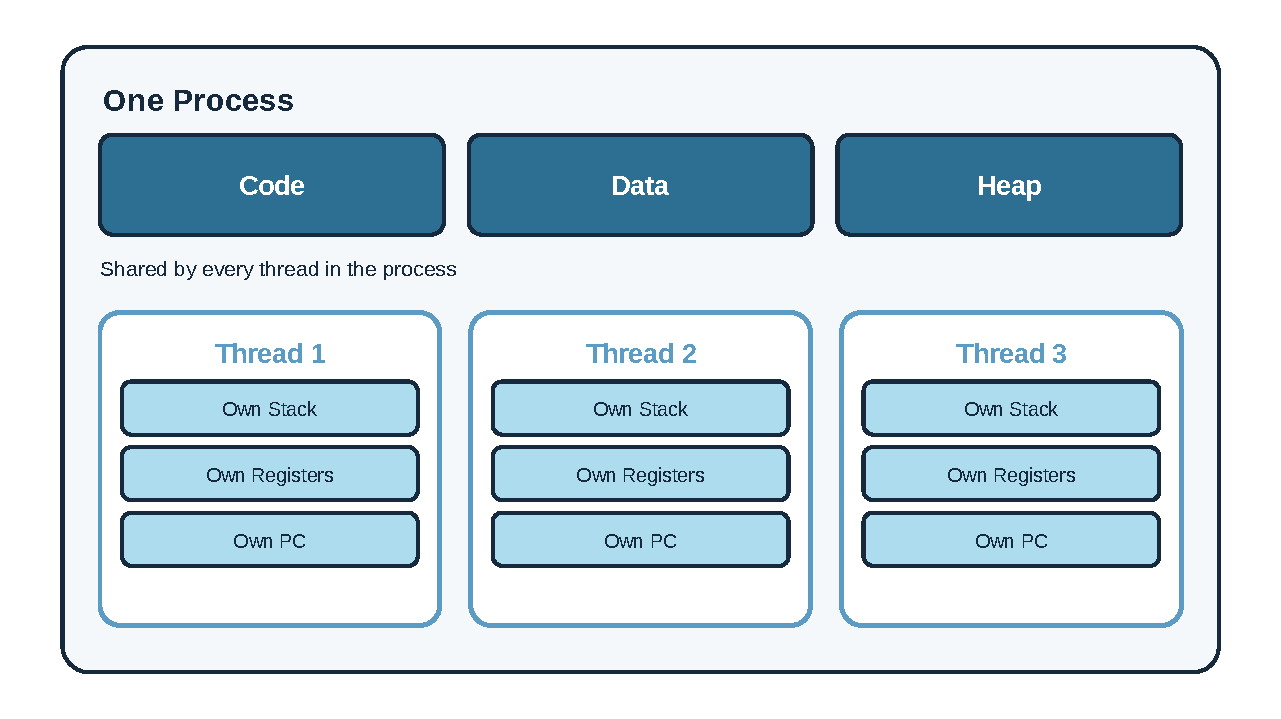
\includegraphics[width=\textwidth]{Images/Chapter9/process-vs-thread.pdf}
    \caption{A process and its threads: shared code/data/heap, but a private stack, registers, and program counter per thread.}
    \label{fig:process-vs-thread}
\end{figure} %[cite: 6]

\begin{table}[h!]
\centering
\small
\renewcommand{\arraystretch}{1.3}
\begin{tabular}{|>{\raggedright\arraybackslash}p{4cm}|>{\raggedright\arraybackslash}p{5cm}|>{\raggedright\arraybackslash}p{5cm}|}
\hline
\textbf{Feature} & \textbf{Process} & \textbf{Thread} \\ \hline
Memory Space & Completely separate & Fully shared with other threads \\ \hline
System Resources & Separate (files, sockets, etc.) & Shared \\ \hline
Creation \& Context Switch Overhead & High & Very low \\ \hline
Independence & Fully independent & Dependent on parent process \\ \hline
Communication Speed & Slow (requires IPC) & Very fast (shared memory) \\ \hline
\end{tabular}
\caption{Comparison of Processes and Threads}
\label{tab:process-vs-thread}
\end{table} %[cite: 6]

\textbf{Advantages of Multithreading:} %[cite: 6]
\begin{itemize}
    \item True parallelism on multi-core CPUs. %[cite: 6]
    \item Better responsiveness (e.g.\ a UI stays active while background work runs on another thread). %[cite: 6]
    \item Easy and fast data sharing between threads (no IPC needed, since memory is already shared). %[cite: 6]
    \item Much lower memory and creation overhead than spawning separate processes. %[cite: 6]
    \item Higher throughput in servers (e.g.\ handling one client request per thread). %[cite: 6]
\end{itemize}
That shared memory is also exactly what makes multithreading dangerous without care -- Section~\ref{sec:race-condition} shows what goes wrong when two threads touch the same data without coordinating. %[cite: 6]

\section{POSIX Threads (pthread)} %[cite: 6]
\texttt{pthread} is the standard POSIX Threads library for multithreaded programming on Unix/Linux systems. %[cite: 6] It is portable, widely used, and available on all Linux distributions and macOS. %[cite: 6]

\textbf{To use pthread in C:} %[cite: 6]
\begin{lstlisting}[language=C]
#include <pthread.h>
\end{lstlisting} %[cite: 6]

\textbf{Compile with the pthread flag:} %[cite: 6]
\begin{lstlisting}[language=Terminal]
$ gcc -pthread program.c -o program
\end{lstlisting} %[cite: 6]
\textbf{Note:} the \texttt{-pthread} flag is required at compile time even though you only \texttt{\#include}d the header -- without it, the linker won't pull in the actual pthread implementation. %[cite: 6]

\textbf{Main pthread Functions:} %[cite: 6]
\begin{table}[h!]
\centering
\small
\renewcommand{\arraystretch}{1.3}
\begin{tabular}{|>{\raggedright\arraybackslash}p{5cm}|>{\raggedright\arraybackslash}p{9cm}|}
\hline
\textbf{Function} & \textbf{Description} \\ \hline
\texttt{pthread\_create()} & Creates a new thread and starts executing the specified function \\ \hline
\texttt{pthread\_join()} & Waits for the specified thread to terminate \\ \hline
\texttt{pthread\_exit()} & Terminates the calling thread \\ \hline
\texttt{pthread\_self()} & Returns the ID of the calling thread \\ \hline
\texttt{pthread\_detach()} & Detaches a thread (its resources are reclaimed automatically on exit) \\ \hline
\texttt{pthread\_mutex\_init()} & Initializes a mutex \\ \hline
\texttt{pthread\_mutex\_lock()} & Locks a mutex (blocks if it is already locked) \\ \hline
\texttt{pthread\_mutex\_unlock()} & Unlocks a mutex \\ \hline
\texttt{pthread\_mutex\_destroy()} & Destroys a mutex after use \\ \hline
\end{tabular}
\caption{Common pthread Functions}
\label{tab:pthread-functions}
\end{table} %[cite: 6]

\textbf{Simple Example: Creating One Thread} %[cite: 6]
\begin{lstlisting}[language=C]
#include <pthread.h>
#include <stdio.h>

void* my_thread(void* arg) {
    printf("Hello from the new thread!\n");
    return NULL;
}

int main() {
    pthread_t tid;

    pthread_create(&tid, NULL, my_thread, NULL);  // Create thread
    pthread_join(tid, NULL);                      // Wait for thread to finish

    printf("Main thread finished.\n");
    return 0;
}
\end{lstlisting} %[cite: 10]

\textbf{Output:} %[cite: 6]
\begin{lstlisting}[language=Terminal]
Hello from the new thread!
Main thread finished.
\end{lstlisting} %[cite: 6]

\textbf{Analysis:} %[cite: 6]
\begin{itemize}
    \item The thread function must return \texttt{void*} and accept \texttt{void*} -- a generic signature that lets you pass and return any kind of data. %[cite: 6]
    \item \texttt{pthread\_create} hands back the new thread's ID through an output pointer, rather than as its return value (which instead reports success or failure). %[cite: 6]
    \item \texttt{pthread\_join} is essential -- without it, if \texttt{main} exits first, the whole program terminates and the child thread is killed along with it, whether or not it had finished. %[cite: 6]
\end{itemize}

\textbf{Practical Example: Multiple Threads Doing Different Tasks} %[cite: 6]
\begin{lstlisting}[language=C]
#include <pthread.h>
#include <stdio.h>
#include <unistd.h>

void* hello(void* arg) {
    for (int i = 0; i < 5; i++) {
        printf("Hello\n");
        sleep(1);
    }
    return NULL;
}

void* world(void* arg) {
    for (int i = 0; i < 5; i++) {
        printf("      World\n");
        sleep(1);
    }
    return NULL;
}

void* count(void* arg) {
    for (int i = 1; i <= 5; i++) {
        printf("            Counter: %d\n", i);
        sleep(1);
    }
    return NULL;
}

int main() {
    pthread_t t1, t2, t3;

    pthread_create(&t1, NULL, hello, NULL);
    pthread_create(&t2, NULL, world, NULL);
    pthread_create(&t3, NULL, count, NULL);

    pthread_join(t1, NULL);
    pthread_join(t2, NULL);
    pthread_join(t3, NULL);

    printf("All threads finished.\n");
    return 0;
}
\end{lstlisting} %[cite: 9]

\textbf{Sample (interleaved) output:} %[cite: 6]
\begin{lstlisting}[language=Terminal]
Hello
      World
            Counter: 1
Hello
      World
            Counter: 2
...
\end{lstlisting} %[cite: 6]
This shows real concurrency -- the output order is unpredictable, because the threads are genuinely running at the same time (or being rapidly interleaved on a single core), not one after another. %[cite: 6]

\section{Race Condition Problem} %[cite: 6]
\label{sec:race-condition} %[cite: 6]
When multiple threads modify a shared variable without synchronization, their updates can interfere with each other: %[cite: 6]
\begin{lstlisting}[language=C]
#include <pthread.h>
#include <stdio.h>

int counter = 0;

void* worker(void* arg) {
    for(int i = 0; i < 1000000; i++)
        counter++;      // <- Dangerous! Race condition
    return NULL;
}

int main() {
    pthread_t t1, t2;
    pthread_create(&t1, NULL, worker, NULL);
    pthread_create(&t2, NULL, worker, NULL);
    pthread_join(t1, NULL);
    pthread_join(t2, NULL);

    printf("Final counter: %d\n", counter);   // Usually < 2000000
    return 0;
}
\end{lstlisting} %[cite: 7]

\textbf{What do we expect from this program?} %[cite: 6]
\begin{enumerate}
    \item We have two threads, each calling the same function (\texttt{worker}). %[cite: 6]
    \item Each of them increments the \texttt{counter} variable by one, 1{,}000{,}000 times. %[cite: 6]
    \item At the end we print the variable and expect to see 2{,}000{,}000. %[cite: 6]
    \item But the actual answer is always \emph{less than} 2{,}000{,}000. %[cite: 6]
\end{enumerate}

\textbf{Why?} The statement \texttt{counter++} is not atomic -- it actually consists of three separate steps: %[cite: 6]
\begin{enumerate}
    \item Read \texttt{counter}. %[cite: 6]
    \item Increment the value. %[cite: 6]
    \item Write the new value back. %[cite: 6]
\end{enumerate}
If two threads interleave these steps, they can both read the \emph{same} old value before either writes back -- so one thread's increment is silently lost. %[cite: 6] Figure~\ref{fig:race-condition} (top panel) walks through exactly this scenario. %[cite: 6]

\begin{figure}[h]
    \centering
    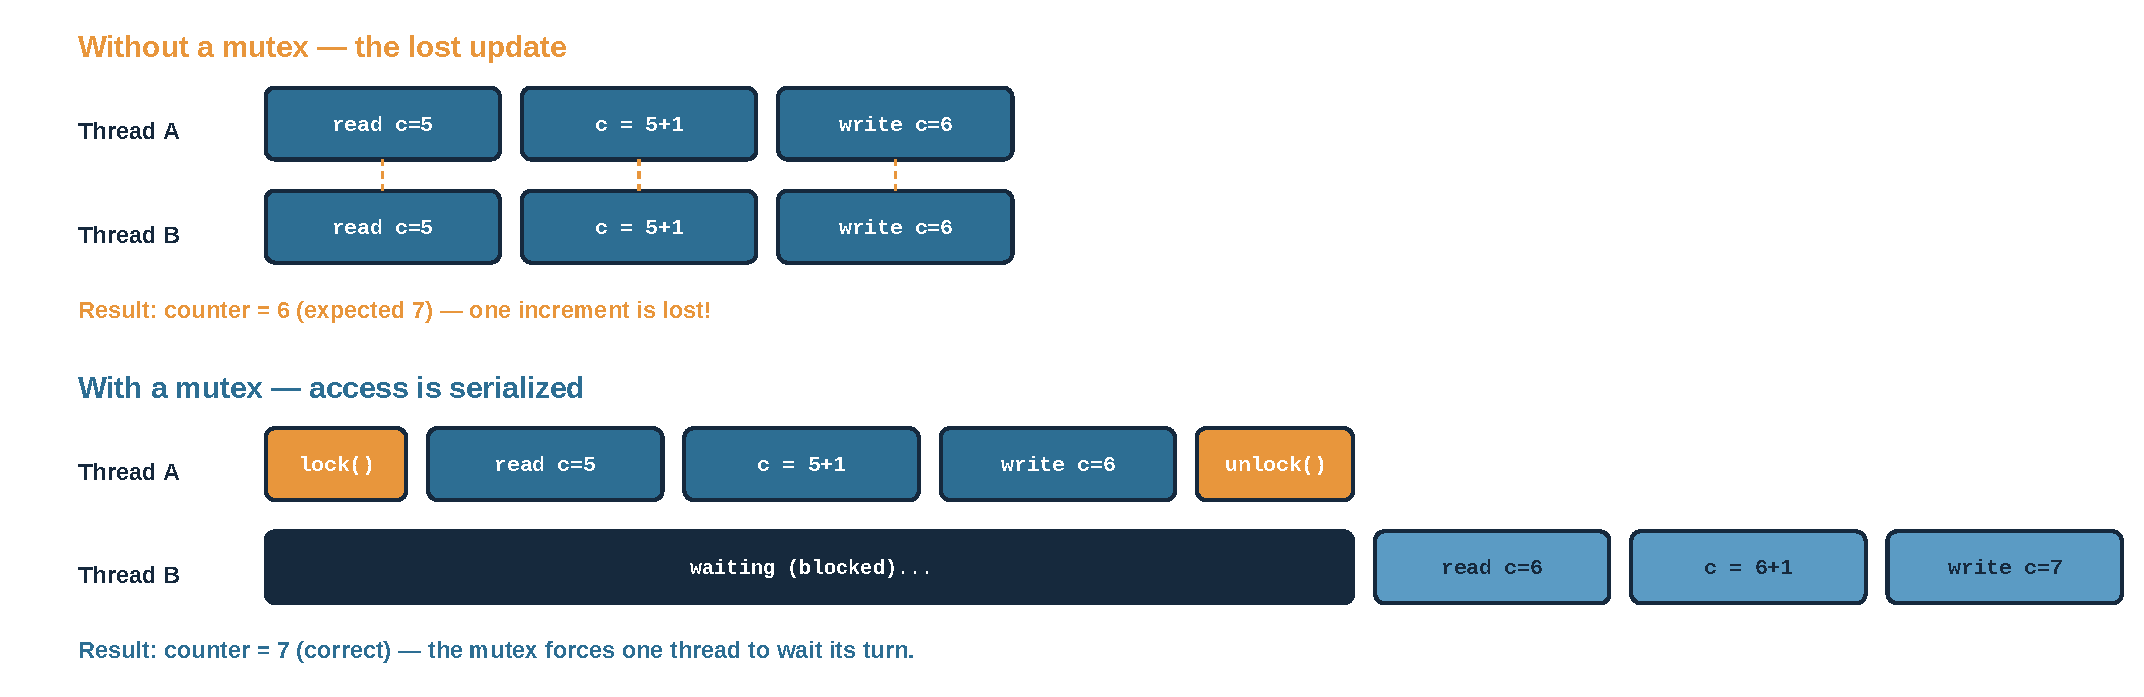
\includegraphics[width=\textwidth]{Images/Chapter9/race-condition.pdf}
    \caption{The same read-increment-write sequence, without synchronization (top, a lost update) and with a mutex (bottom, correctly serialized).}
    \label{fig:race-condition}
\end{figure} %[cite: 6]

\subsection{Solving Race Conditions with a Mutex} %[cite: 6]
To prevent race conditions, we need a synchronization mechanism that ensures only one thread at a time can access a shared resource -- the section of code touching that resource is called the \textbf{critical section}. %[cite: 6] Common tools include mutexes, semaphores, condition variables, and atomic operations. %[cite: 6]

The most frequently used and simplest of these is a \textbf{mutex} (short for ``mutual exclusion''). %[cite: 6]

A mutex is a lock that protects a critical section of code. %[cite: 6] Before entering the critical section, a thread calls \texttt{pthread\_mutex\_lock()}. %[cite: 6] If another thread already holds the lock, the calling thread blocks (sleeps) until the lock is released with \texttt{pthread\_mutex\_unlock()}. %[cite: 6] This guarantees that only one thread executes the protected code at any given time, eliminating the race condition -- exactly as shown in the bottom panel of Figure~\ref{fig:race-condition}. %[cite: 6]

\begin{lstlisting}[language=C]
#include <pthread.h>
#include <stdio.h>

int counter = 0;
pthread_mutex_t lock = PTHREAD_MUTEX_INITIALIZER;

void* worker_safe(void* arg) {
    for(int i = 0; i < 1000000; i++) {
        pthread_mutex_lock(&lock);    // Only one thread can enter
        counter++;
        pthread_mutex_unlock(&lock);  // Release lock
    }
    return NULL;
}

int main() {
    pthread_t t1, t2;
    pthread_create(&t1, NULL, worker_safe, NULL);
    pthread_create(&t2, NULL, worker_safe, NULL);
    pthread_join(t1, NULL);
    pthread_join(t2, NULL);

    printf("Final counter: %d\n", counter);   // Always exactly 2000000
    return 0;
}
\end{lstlisting} %[cite: 8]

\textbf{Analysis:} %[cite: 6]
\begin{itemize}
    \item The critical section (the increment) is protected by the mutex. %[cite: 6]
    \item Only one thread at a time can execute it, so no update is ever lost. %[cite: 6]
    \item Correctness is guaranteed, at the cost of a small performance overhead -- every other thread has to wait its turn instead of running freely. %[cite: 6]
\end{itemize}

\newpage %[cite: 6]
\section{Hands-on Tasks} %[cite: 6]
This assignment should be completed in class and graded by the course instructor or teaching assistants. %[cite: 6]

\textbf{Task 1:}\\ %[cite: 6]
Create two threads. One prints \texttt{"Hello"} and the other prints \texttt{"World"}, 5 times each. %[cite: 6]
\begin{itemize}
    \item Each thread should print its message 5 times with a slight delay (\texttt{sleep(1)}). %[cite: 6]
    \item Ensure \texttt{main} waits for both threads to finish before exiting. %[cite: 6]
\end{itemize}

\vspace{0.5cm} %[cite: 6]

\textbf{Task 2:}\\ %[cite: 6]
Use two threads to compute the sum of two halves of a given array, then compute the total sum in \texttt{main}. %[cite: 6]
\begin{itemize}
    \item Split the array into two (roughly equal) halves and give each thread its own start index and length -- for example, by passing a small \texttt{struct} to each thread via \texttt{pthread\_create}'s argument pointer. %[cite: 6]
    \item Have each thread store its partial sum somewhere \texttt{main} can read after joining both threads (e.g.\ through that same struct, or a return value passed via \texttt{pthread\_exit}). %[cite: 6]
\end{itemize}

\vspace{0.5cm} %[cite: 6]

\textbf{Task 3:}\\ %[cite: 6]
Create 5 threads that each increment a shared counter 1000 times, using a \texttt{mutex} for synchronization.\\ %[cite: 6]
\textbf{Objective:} understand race conditions and synchronization with \texttt{pthread\_mutex\_t}. %[cite: 6]
\begin{itemize}
    \item It makes sense to use a global counter variable, protected by a global mutex. %[cite: 6]
    \item At the end, print the final value (it should be exactly 5000). %[cite: 6]
\end{itemize}